\documentclass[12pt]{article}

\usepackage{sbc-template}
\usepackage{float} % Pacote para a opção [H]
\usepackage{graphicx,url}


\usepackage[brazil]{babel}   
\usepackage[utf8]{inputenc}  

     
\sloppy

\title{Artigo de Software Back-end}

\author{Daniella Ferreira Marques}


\address{Instituto Federal do Piauí - IFPI - Campus Picos
\email{isabelmarques902@gmail.com}
}

\begin{document} 

\maketitle

\begin{abstract}
  Tradução do texto original para o inglês.   
  
  \textbf{Keywords:}
\end{abstract}
     
\begin{resumo}
   Para a elaboração do resumo e do abstract em um trabalho acadêmico, é recomendado utilizar fontes como Arial ou Times New Roman, tamanho 12, com espaçamento entre linhas simples de 1,0. É importante que o resumo contenha entre 150 a 250 palavras, incluindo informações sobre os objetivos do estudo, fundamentação teórica, metodologia, resultados e conclusões ou considerações. É fundamental que o texto não contenha citações ou siglas.  

   
   \textbf{Palavras - chave:} O documento requer a inclusão de um conjunto de descritores composto por um mínimo de três e um máximo de cinco termos, cujas letras iniciais devem ser grafadas em minúsculo, separados por ponto e vírgula, e terminados com um ponto final.
\end{resumo}


\section{Introdução}

Ao escrever a introdução de um artigo, é importante incluir informações essenciais para contextualizar o leitor sobre o que será abordado na pesquisa. As três principais partes que devem ser incluídas são o tema, o problema e a hipótese.

O tema do artigo é o assunto principal que será abordado na pesquisa. Ele deve ser claro e objetivo, de modo que o leitor possa compreender imediatamente sobre o que será tratado no artigo. O problema de pesquisa, por sua vez, é a questão que motivou a realização do estudo. É importante que o problema seja apresentado de forma clara e objetiva, indicando qual é a questão que será investigada e a importância de se estudar tal questão. A hipótese é uma suposição inicial que o pesquisador faz sobre a relação entre as variáveis em estudo. Ela deve ser baseada em evidências científicas e ter uma relação clara com o problema de pesquisa.

Por fim, a introdução deve apresentar a estrutura do artigo, indicando como o estudo foi organizado e quais são os principais pontos abordados em cada seção. Isso ajuda o leitor a se orientar durante a leitura. É importante que o tema, o problema e a hipótese sejam apresentados de forma simples e clara, que a relevância do tema seja destacada, que o escopo da pesquisa seja delimitado e que a estrutura do artigo seja apresentada.

\section{Metodologia} \label{sec:firstpage}
Ao planejar o desenvolvimento de uma plataforma, é essencial considerar diversos requisitos estratégicos, como tecnologias utilizadas, volume de acessos, usabilidade, escalabilidade e confiabilidade. Com o objetivo de criar uma plataforma simples e eficiente, o processo pode ser desenvolvimento em três etapas distintas:
   \begin{itemize}
       \item Etapa inicial de desenvolvimento: Nessa fase, a plataforma é construída, levando em conta os requisitos e as tecnologias escolhidas. A equipe de desenvolvimento se concentra na implementação das funcionalidades principais e na criação da estrutura básica da plataforma.
       \item Testes: Após a conclusão da etapa de desenvolvimento, são realizados testes para identificar e corrigir possíveis erros de código. Esses testes visam garantir a qualidade e a estabilidade da plataforma, verificando se ela funciona conforme o esperado e atende aos requisitos definidos.
       \item Validação com usuários finais: Nessa etapa, a plataforma é submetida à validação por parte dos usuários finais. O foco é avaliar a usabilidade, confiabilidade e efetividade da plataforma. Os usuários são convidados a interagir com a plataforma, realizar tarefas específicas e fornecer feedback sobre sua experiência. Essa validação ajuda a identificar possíveis melhorias e a garantir que a plataforma atenda às necessidades dos usuários de forma eficiente.
   \end{itemize}

\section{Estado da Arte}
O estado da arte é basicamente o que há de mais avançado em uma determinada área de pesquisa. É importante para os pesquisadores entenderem o que já foi feito e quais questões ainda precisam ser respondidas. Isso ajuda a escolher a melhor metodologia e ferramentas, e também dá contexto aos resultados.

Para descobrir o estado da arte de um software, é preciso estudar a literatura existente, pesquisar as tecnologias mais novas e aprender com as boas práticas recomendadas na área de interesse. Isso permite ter uma visão geral das tendências e inovações no desenvolvimento de software e aplicar o conhecimento adquirido para criar softwares mais eficientes e de qualidade. O estado da arte de um determinado produto ou tecnologia pode ser dividido em dois tipos: concorrentes diretos e indiretos.
\subsection{Concorrentes Diretos}
Os concorrentes diretos são aqueles que oferecem produtos ou tecnologias que têm o mesmo objetivo ou função do produto em questão. Por exemplo, se o produto em questão é um smartphone, seus concorrentes diretos são outros smartphones no mercado.
\subsection{Concorrentes Indiretos}
Concorrentes indiretos são produtos ou soluções que oferecem funcionalidades ou benefícios semelhantes, mas que não competem diretamente com o software em questão. Eles podem estar em diferentes setores ou mercados, mas ainda assim podem impactar a adoção ou utilização do software em questão. Por exemplo, se o produto é um smartphone, seus concorrentes indiretos são o e-reader (leitor de livros digitais). Embora os smartphones possam oferecer aplicativos de leitura de livros, os e-readers são dispositivos eletrônicos dedicados para esse fim, oferecendo uma experiência de leitura mais confortável para os usuários. 

\section{Arquitetura de software}\label{sec:figs}
A seção de arquitetura do software fornece uma visão geral da estrutura do sistema, destacando seus principais componentes e como eles interagem entre si. Ela descreve a arquitetura em alto nível, incluindo os padrões arquiteturais utilizados e as principais decisões tomadas durante o projeto do sistema. Além disso, aborda os componentes do sistema, sua comunicação e integração, o gerenciamento de dados, a escalabilidade e o desempenho, a segurança e as considerações de implantação. Essa seção é crucial para compreender a organização do software e como ele atende aos requisitos do sistema, garantindo a qualidade,  e eficiência da aplicação.

\subsection{API}
Na seção da API, são apresentadas a finalidade e funcionalidades da API, listando os endpoints disponíveis com seus métodos HTTP correspondentes. São abordados temas como autenticação, autorização, formato de dados e códigos de status HTTP. É útil fornecer exemplos de solicitações e respostas, além de tratar de versionamento, limites, tratamento de erros e documentação adicional. Essa seção serve como um guia completo para os desenvolvedores que desejam utilizar a API, oferecendo todas as informações necessárias para uma integração correta e efetiva em seus projetos.

\subsection{Visão lógica}
Na visão lógica, são apresentados os principais componentes do sistema, suas responsabilidades e interações. Isso pode ser feito através de diagramas, modelos ou descrições textuais. O objetivo é fornecer uma representação clara e concisa da estrutura e do fluxo de informações dentro do sistema, sem se aprofundar em detalhes de implementação.

\subsection{Visão de caso de uso}
A visão de caso de uso é uma parte do documento de arquitetura que descreve como os usuários interagem com o sistema, identificando os casos de uso principais, descrevendo suas ações, entradas e saídas esperadas, e apresentando o fluxo de eventos. Essa visão é importante para compreender as necessidades dos usuários e fornecer uma base sólida para o design e a implementação do sistema. A figura 1 ilustra um modelo de caso de uso de negócio.
\begin{figure}[ht]
\centering
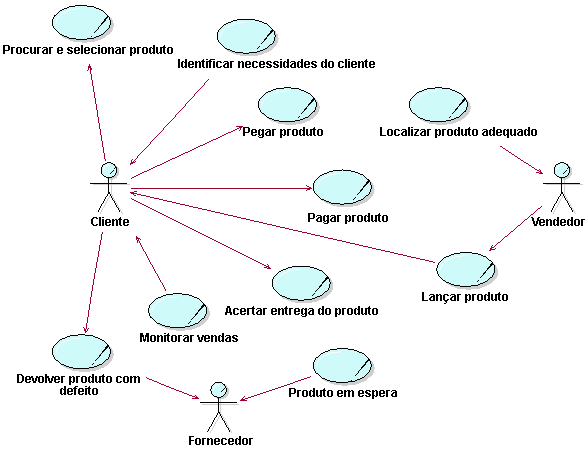
\includegraphics[width=.7\textwidth, scale=6.7]{caso.png}
\caption{Exemplo de um caso de uso de negócio}
\label{fig:typical-figure}
\end{figure}

\subsection{Modelo de entidade relacionamento}
O Modelo de Entidade-Relacionamento (MER) é uma técnica visual usada para representar a estrutura de dados de um sistema. Ele usa retângulos para representar entidades, linhas para mostrar relacionamentos e atributos para descrever informações específicas. É uma ferramenta útil no projeto de bancos de dados, permitindo uma compreensão clara das entidades, relacionamentos e atributos envolvidos no sistema. O Diagrama de Entidade-Relacionamento é uma representação visual que possui três componentes principais: entidades, atributos e relacionamentos.
\begin{itemize}
    \item Entidades são os objetos ou conceitos relevantes do domínio do problema que serão armazenados no banco de dados. Elas são representadas por retângulos no diagrama, como estudantes, professores e cursos.
    \item Atributos são as propriedades ou características das entidades, fornecendo informações adicionais sobre elas. São representados por elipses conectadas às entidades correspondentes. Exemplos de atributos são nome, endereço e número de matrícula de um estudante.
    \item Relacionamentos indicam as associações entre as entidades, mostrando como elas se conectam entre si. São representados por losangos no diagrama. Por exemplo, um relacionamento "inscrição" pode existir entre estudantes e cursos, indicando que um estudante está inscrito em um curso.
\end{itemize}
\begin{figure}[ht]
\centering
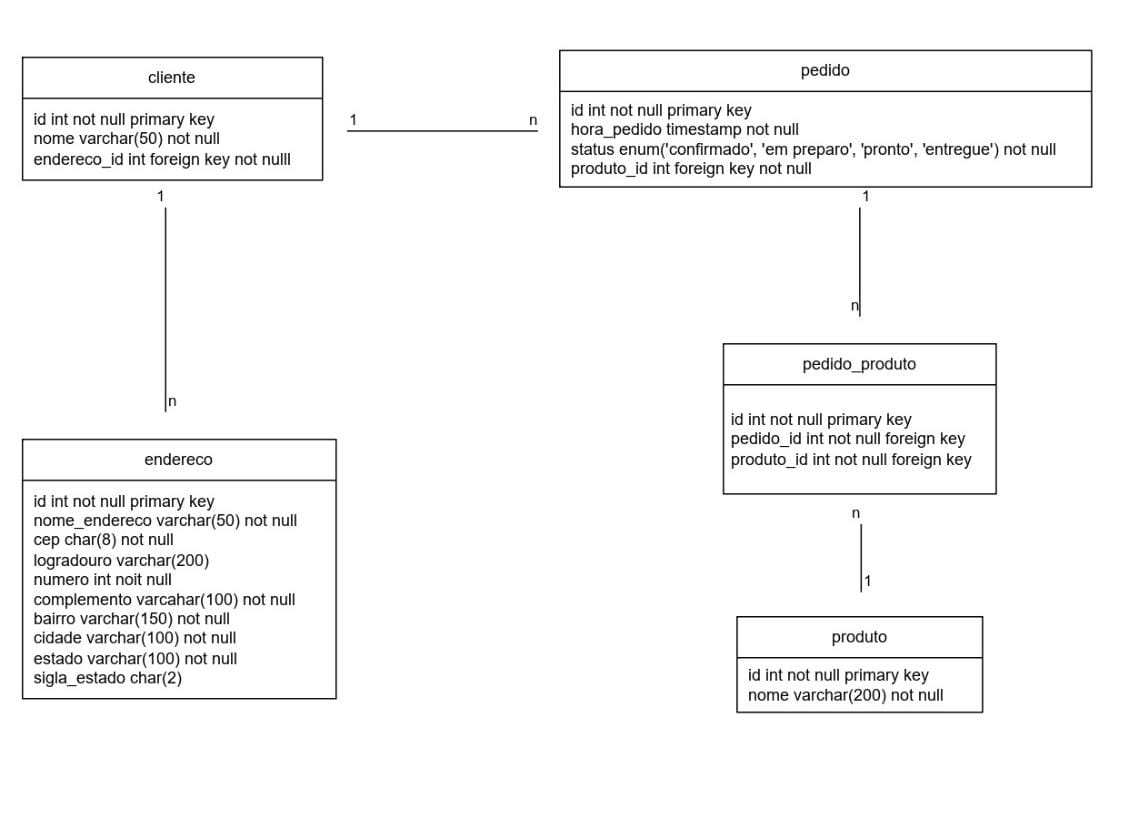
\includegraphics[width=.8\textwidth, scale=6.7]{modelo1.jpeg}
\caption{Exemplo de entidade-relacionamento para um sistema de pedidos}
\label{fig:typical-figure}
\end{figure}

\section{Protótipo do software}
Um protótipo de software é uma versão inicial ou funcional de um software em desenvolvimento. Ele é criado para validar ideias, testar funcionalidades e obter feedback dos usuários antes do desenvolvimento completo. Existem diferentes abordagens, desde protótipos de baixa fidelidade até protótipos de alta fidelidade. O objetivo é identificar problemas e refinar o software antes de investir recursos no desenvolvimento completo, resultando em um produto final mais sólido e satisfatório.

\subsection{Protótipos de alta fidelidade}
 Nesse método, são usadas ferramentas de design e desenvolvimento mais avançadas para criar protótipos com aparência e interações próximas às do produto final. Isso pode incluir o uso de ferramentas de design gráfico, como o Adobe XD, Sketch ou Figma, para criar layouts e interfaces mais elaboradas, bem como adicionar interações e animações para simular o comportamento do software.
 
 \subsection{Repositório}
Incluir o link do repositório do software no artigo é uma prática comum e útil para que os leitores possam acessar e explorar o código-fonte do projeto. Além disso, também facilita a colaboração e contribuição da comunidade. Ao mencionar o repositório, você pode adicionar uma frase como esta:

"O código-fonte completo do software desenvolvido pode ser encontrado no repositório do projeto, disponível em [inserir link do repositório]. Neste repositório, os interessados têm acesso ao código, documentação adicional e podem contribuir com sugestões, correções ou novas funcionalidades."

Lembre-se de substituir "[inserir link do repositório]" pelo link real do repositório onde o software está hospedado, como GitHub, GitLab ou qualquer outra plataforma de controle de versão utilizada para o projeto. Isso permitirá que os leitores acessem diretamente o repositório para obter mais informações e interagir com o código-fonte.

\section{Avaliação}
Nesta seção, serão apresentados os testes de infraestrutura e usabilidade realizados, bem como os resultados obtidos, visando assegurar a confiabilidade, usabilidade e integridade do sistema.

\subsection{Teste de desempenho}
O teste de desempenho avalia o desempenho, estabilidade e escalabilidade de um sistema em condições de carga e estresse. Simula situações reais com muitos usuários ou carga intensiva, analisando o tempo de resposta, taxa de transferência, capacidade de processamento e utilização de recursos. Identificando gargalos e pontos fracos, o teste permite otimizar o sistema, ajustar configurações e melhorar a experiência do usuário. Existem várias ferramentas gratuitas disponíveis para realizar testes de desempenho. Aqui estão alguns exemplos:
\begin{itemize}
   \item Page Speed Insights (O Google PageSpeed: É
uma família de ferramentas do Google Inc, projetada para ajudar na otimização do
desempenho de um site), com esta ferramenta é possível identificar problemas de
codificação, usabilidade, carregamento de páginas e renderização das páginas para
dispositivos de telas diferentes. 
\item Apache JMeter: É uma ferramenta de teste de carga e desempenho amplamente utilizada. Permite simular diferentes cargas de trabalho, medir o desempenho de servidores web, aplicativos e serviços, além de oferecer recursos avançados de relatórios e análise
 \end{itemize}
 
\subsection{Teste de usabilidade}
O teste de usabilidade avalia a facilidade de uso e a experiência do usuário em um produto. Os usuários realizam tarefas enquanto são observados por especialistas. Os resultados identificam problemas e ajudam a melhorar o design e a interação. O teste de usabilidade pode ser realizado seguindo algumas etapas básicas:
\begin{itemize}
   \item Defina os objetivos: Determine quais aspectos do produto você deseja avaliar e quais perguntas deseja responder por meio do teste de usabilidade.
   \item  Identifique o público-alvo: Selecione os usuários que representam o público-alvo do produto. Eles devem ter características que reflitam os usuários reais do produto.
    \item Crie cenários de teste: Desenvolva tarefas ou cenários realistas que os usuários devem realizar durante o teste. Essas tarefas devem abranger os principais recursos e funcionalidades do produto.
    \item Execute o teste: Peça aos usuários selecionados que realizem as tarefas definidas enquanto são observados. Encoraje-os a pensar em voz alta e expressar suas opiniões e dificuldades durante o processo.
    \item Colete feedback e observe: Registre os comentários, observações e comportamentos dos usuários durante o teste. Observe suas ações, reações e expressões faciais para obter insights adicionais.
    \item Analise os resultados: Revise os dados coletados e identifique os padrões, problemas de usabilidade e oportunidades de melhoria. Priorize as áreas que necessitam de ajustes.
\end{itemize}
\subsection{Resultados}
Ao apresentar os resultados obtidos com os testes de usabilidade, é importante destacar os principais insights e descobertas que foram identificados. Aqui estão algumas informações que podem ser abordadas:
\begin{itemize}
    \item Problemas de usabilidade: Descreva os principais problemas ou dificuldades encontrados pelos usuários durante o teste. Isso pode incluir problemas de navegação, falta de clareza nas instruções, confusão de layout, dificuldade em encontrar informações ou executar tarefas específicas. Forneça exemplos concretos e ilustrativos desses problemas.
    \item Feedback dos usuários: Apresente os comentários, opiniões e sugestões dos usuários durante o teste. 
    \item Ações corretivas tomadas: Descreva as medidas corretivas que foram adotadas com base nos resultados dos testes de usabilidade.
\end{itemize}
\section{Considerações Finais}
Nesta seção, apresentaremos um resumo dos principais pontos do relatório, reafirmando o problema identificado, a solução proposta e discutindo as implicações do trabalho. Além disso, sugeriremos possíveis direções para futuros desenvolvimentos. 

\section{Referências}
\bibliographystyle{sbc}
\bibliography{sbc-template}

\end{document}